\section{更新的接受}
\label{sec:sqp-acceptance}

QP给出的步只在模型里是好的。把步放回非线性问题，凭什么判断它值得采用？

无约束时这个问题很简单，看目标有没有下降。约束问题有两个指标。第~\ref{sec:sqp-equality-qp}节的第三步目标从$-2.0588$升到$-2.0009$，约束违反却从$0.119$降到$0.0018$；而从圆上的点$(1.4,0.2)^\top$走一个全步，目标从$-1.6$降到$-2.32$，违反量却从$0$升到$0.72$。两个指标常常冲突，必须有一条明确规则来评价进展。第~\ref{sec:sqp-merit}小节把两者压成一个数，第~\ref{sec:sqp-filter}小节把两者并排比较。

记约束的总违反量为
\begin{equation}
 \theta(\bm{x})=\sum_{j=1}^p\lvert h_j(\bm{x})\rvert+\sum_{i=1}^m[g_i(\bm{x})]_+,
 \label{eq:sqp-violation}
\end{equation}
其中$[u]_+=\max\{u,0\}$。

\subsection{罚函数线搜索}
\label{sec:sqp-merit}

\paragraph{评价函数}
把目标和违反量加起来，用一个权重$\rho>0$换算两者的单位，得到
\begin{equation}
 \phi_\rho(\bm{x})=f(\bm{x})+\rho\,\theta(\bm{x}).
 \label{eq:sqp-merit}
\end{equation}
这是第~\ref{chap:penalty-multiplier-methods}章的$\ell_1$精确惩罚函数，在这里它的角色是判断步的好坏，称为\term{评价函数}（merit function）。那一章的结论是：若$\bm{x}^\star$满足二阶充分条件，且权重大于乘子的最大绝对值，则$\bm{x}^\star$是$\phi_\rho$的严格局部最小点。乘子是约束的影子价格，权重就是愿意为单位违反付的罚款，罚款低于影子价格，违约反而划算。

$\phi_\rho$在$h_j=0$或$g_i=0$处不可微，但沿任意方向的方向导数存在。记$D(\phi_\rho;\bm{d})$为它在$\bm{x}^{(t)}$处沿$\bm{d}$的方向导数。下面的引理告诉我们，QP的解在什么时候是下降方向。

\begin{lemma}[QP步的下降性]
\label{lem:sqp-merit-descent}
设$(\bm{d},\hat{\bm{\lambda}},\hat{\bm{\nu}})$满足条件~\eqref{eq:sqp-qp-kkt}，则
\begin{equation}
 D(\phi_\rho;\bm{d})\leq-\bm{d}^\top\bm{B}^{(t)}\bm{d}-\bigl(\rho-\max\{\lVert\hat{\bm{\nu}}\rVert_\infty,\lVert\hat{\bm{\lambda}}\rVert_\infty\}\bigr)\theta(\bm{x}^{(t)}).
 \label{eq:sqp-merit-descent}
\end{equation}
\end{lemma}

\begin{proof}
分别计算$\theta$和$f$的方向导数。先看等式项。线性化约束给出$\langle\nabla h_j,\bm{d}\rangle=-h_j$。若$h_j\neq0$，则$\lvert h_j\rvert$的方向导数是$h_j$的符号乘以$\langle\nabla h_j,\bm{d}\rangle$，等于$-\lvert h_j\rvert$；若$h_j=0$，则$\langle\nabla h_j,\bm{d}\rangle=0$，方向导数为$0$。两种情况都等于$-\lvert h_j\rvert$。

再看不等式项，线性化约束给出$\langle\nabla g_i,\bm{d}\rangle\leq-g_i$。若$g_i>0$，$[g_i]_+$的方向导数是$\langle\nabla g_i,\bm{d}\rangle\leq-[g_i]_+$；若$g_i=0$，方向导数是$[\langle\nabla g_i,\bm{d}\rangle]_+=0$；若$g_i<0$，方向导数是$0$。三种情况都不超过$-[g_i]_+$。把这些加起来，得到
\[
 D(\theta;\bm{d})\leq-\theta(\bm{x}^{(t)}).
\]

然后看目标。用$\bm{d}^\top$左乘式~\eqref{eq:sqp-qp-kkt}第一行，再用线性化约束和互补条件换掉$\bm{A}\bm{d}$和$\bm{G}\bm{d}$：
\[
 \begin{aligned}
 \langle\nabla f,\bm{d}\rangle
 &=-\bm{d}^\top\bm{B}\bm{d}-\hat{\bm{\nu}}^\top\bm{A}\bm{d}-\hat{\bm{\lambda}}^\top\bm{G}\bm{d}\\
 &=-\bm{d}^\top\bm{B}\bm{d}+\hat{\bm{\nu}}^\top\bm{h}+\hat{\bm{\lambda}}^\top\bm{g}.
 \end{aligned}
\]

最后估计两个内积。第一个用Hölder不等式，第二个先用$\hat{\bm{\lambda}}\geq\bm{0}$把$\bm{g}$放大成$[\bm{g}]_+$，再用Hölder不等式：
\[
 \begin{aligned}
 \hat{\bm{\nu}}^\top\bm{h}&\leq\lVert\hat{\bm{\nu}}\rVert_\infty\lVert\bm{h}\rVert_1,\\
 \hat{\bm{\lambda}}^\top\bm{g}&\leq\hat{\bm{\lambda}}^\top[\bm{g}]_+\leq\lVert\hat{\bm{\lambda}}\rVert_\infty\lVert[\bm{g}]_+\rVert_1.
 \end{aligned}
\]

合起来，
\[
 \langle\nabla f,\bm{d}\rangle\leq-\bm{d}^\top\bm{B}\bm{d}+\max\{\lVert\hat{\bm{\nu}}\rVert_\infty,\lVert\hat{\bm{\lambda}}\rVert_\infty\}\,\theta(\bm{x}^{(t)}).
\]
$\phi_\rho$的方向导数是$\langle\nabla f,\bm{d}\rangle$与$\rho D(\theta;\bm{d})$之和，式~\eqref{eq:sqp-merit-descent}成立。
\end{proof}

引理说明，当$\rho$超过QP乘子的最大绝对值，并且$\bm{d}^\top\bm{B}\bm{d}$为正时，$\bm{d}$是$\phi_\rho$的下降方向。这里的正性只需在$\bm{d}$上成立。$\bm{d}^\top\bm{B}\bm{d}$可能为负时，条件要通过第~\ref{sec:sqp-curvature}节的修正来保证。

\paragraph{权重的两难}
式~\eqref{eq:sqp-merit-descent}要求$\rho$足够大，但$\rho$并不是越大越好。看问题~\eqref{eq:sqp-circle}沿射线$x_1=x_2=s$的情形，此时
\[
 \phi_\rho(s,s)=-2s+\rho\,\lvert2s^2-2\rvert.
\]

在$s>1$上，$\phi_\rho$的导数是$-2+4\rho s$。$\rho=0.1$时导数在$s=5$才变号，评价函数在$(5,5)$有局部最小值，其值$-5.2$比解处的$-2$还小。沿着$\phi_{0.1}$下降会被带到严重违约的地方。

$s=1$处的右导数是$-2+4\rho$，要它为正需要$\rho>1/2=\nu^\star$，这正是权重要超过乘子的具体含义。图~\ref{fig:sqp-merit-rho-ray}比较了三种权重。权重过大时，$\phi_\rho$在约束面两侧形成很陡的峡谷，任何离开约束面的步，即使只离开$\lVert\bm{d}\rVert_2^2$这么多，也要付很高的代价，步长于是被压得很小，迭代只能贴着约束面慢慢挪。

\begin{BookInlineFigure}
 \centering
 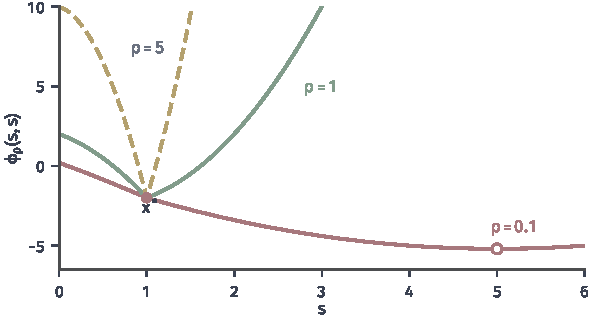
\includegraphics[width=100mm]{figures/05-optimization/06-constrained-optimization/matplotlib/sqp-merit-rho-ray/figure.pdf}
 \caption{评价函数沿射线$x_1=x_2=s$的形状。红线$\rho=0.1$低于乘子，空心点$(5,5)$是错误的局部最小点；绿线$\rho=1$在解$s=1$（红点）处形成拐点；黄色虚线$\rho=5$的峡谷很陡。}
 \label{fig:sqp-merit-rho-ray}
\end{BookInlineFigure}

实际算法动态调整权重。常用规则是每轮令$\rho$不小于当前QP乘子的最大绝对值再加一个裕量$\delta>0$：
\begin{equation}
 \rho^{(t)}\geq\max\{\lVert\hat{\bm{\nu}}\rVert_\infty,\lVert\hat{\bm{\lambda}}\rVert_\infty\}+\delta.
 \label{eq:sqp-rho-rule}
\end{equation}
权重只升不降时，迭代的后期可能一直背着远离解时抬高的权重，因此实现中也允许有控制地下调。

\paragraph{主要思想}
有了下降方向，就和无约束问题一样回溯。从$\alpha=1$开始试，直到满足充分下降条件：
\begin{equation}
 \phi_\rho(\bm{x}^{(t)}+\alpha\bm{d}^{(t)})\leq\phi_\rho(\bm{x}^{(t)})+\eta\,\alpha\,D(\phi_\rho;\bm{d}^{(t)}),
 \label{eq:sqp-armijo}
\end{equation}
其中$\eta\in(0,1/2)$。由于$\phi_\rho$沿$\bm{d}$在$\alpha=0$右侧的导数就是$D$，小的$\alpha$总能满足这个条件。

\needspace{6\baselineskip}
\paragraph{变量}
\begin{itemize}
 \item $\bm{x}^{(t)}$、$\bm{\nu}^{(t)}$：当前点与乘子；$\rho$：评价函数的权重。
 \item $\bm{d}^{(t)}$、$\hat{\bm{\nu}}$：QP的解与乘子；$D$：$\phi_\rho$的方向导数。
 \item $\eta$：充分下降系数；$\alpha^{(t)}$：接受的步长。
\end{itemize}

\paragraph{初始化}
给定$\bm{x}^{(0)}$、$\bm{\nu}^{(0)}$、$\rho$和$\eta$。例中取圆上的一点，数据是
\[
 \bm{x}^{(0)}=(1.4,\ 0.2)^\top,\qquad\nu^{(0)}=0.5,\qquad\rho=2,\qquad\eta=0.1.
\]
这里$h(\bm{x}^{(0)})=1.96+0.04-2=0$，点是可行的，$\phi_\rho(\bm{x}^{(0)})=-1.6$。

\needspace{6\baselineskip}
\paragraph{每轮更新}
\begin{enumerate}
 \item 解QP得$\bm{d}^{(t)}$和乘子。例中第一轮$\bm{B}=\bm{I}$，$\bm{A}=(2.8,0.4)$，$h=0$，解得
 \[
  \hat\nu=0.4,\qquad\bm{d}^{(0)}=(-0.12,\ 0.84)^\top.
 \]

 \item 按需要增大$\rho$，并计算方向导数，即$D=\langle\nabla f,\bm{d}\rangle-\rho\,\theta$（只含等式时）。例中$\rho=2\geq\hat\nu$，$\theta=0$，于是
 \[
  D=\langle(-1,-1)^\top,\bm{d}^{(0)}\rangle=-0.72.
 \]

 \item 令$\alpha=1$，当式~\eqref{eq:sqp-armijo}不成立时令$\alpha\leftarrow\alpha/2$。例中沿$\bm{d}$有$h(\bm{x}+\alpha\bm{d})=0.72\alpha^2$，$f(\bm{x}+\alpha\bm{d})=-1.6-0.72\alpha$，所以
 \[
  \phi_\rho(\alpha)=-1.6-0.72\,\alpha+1.44\,\alpha^2.
 \]

 依次试三个步长，每个步长下左边是$\phi_\rho$的值，右边是式~\eqref{eq:sqp-armijo}的门槛：
 \[
  \begin{aligned}
  \alpha=1:&\quad-0.88>-1.672,\\
  \alpha=0.5:&\quad-1.6>-1.636,\\
  \alpha=0.25:&\quad-1.69\leq-1.618.
  \end{aligned}
 \]
 前两个被拒绝，第三个被接受，图~\ref{fig:sqp-merit-armijo}画出了这三次试探。

 \item 更新迭代点，乘子按式~\eqref{eq:sqp-multiplier-update}。例中第一轮
 \[
  \bm{x}^{(1)}=(1.37,\ 0.41)^\top,\qquad\nu^{(1)}=0.5+0.25\,(0.4-0.5)=0.475.
 \]

 第二轮$h=0.045$，$\bm{d}^{(1)}\approx(-0.21767,0.67247)^\top$，$\alpha^{(1)}=0.25$；第三轮$\alpha^{(2)}=0.5$；第四轮起$\alpha^{(t)}=1$。

 \item 按第~\ref{sec:sqp-convergence}节的残差判断是否停止。
\end{enumerate}

最终$\bm{x}^{(t)}$到达$(1,1)^\top$，例中$t=6$时到解的距离已低于$10^{-6}$。

\begin{BookInlineFigure}
 \centering
 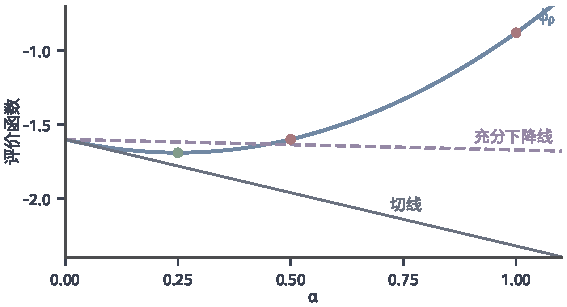
\includegraphics[width=96mm]{figures/05-optimization/06-constrained-optimization/matplotlib/sqp-merit-armijo/figure.pdf}
 \caption{从$\bm{x}^{(0)}=(1.4,0.2)^\top$沿QP步的评价函数，$\rho=2$。蓝线是$\phi_\rho(\alpha)$，灰线是切线，紫色虚线是充分下降的门槛。红点$\alpha=1$与$\alpha=0.5$被拒绝，绿点$\alpha=0.25$被接受。}
 \label{fig:sqp-merit-armijo}
\end{BookInlineFigure}

这个例子还暗示了一个毛病。全步到达$(1.28,1.04)^\top$，到解的距离从$0.894$缩到$0.283$，明明很好，评价函数却把它拒绝了。原因及补救在第~\ref{sec:sqp-soc}小节。

\paragraph{用信赖域代替线搜索}
线搜索固定方向、调整步长。也可以用第~\ref{chap:trust-region}章的方式固定一个半径，比较实际下降与模型预测，比值大则接受并放大半径，比值小则缩小半径。线性化的约束有可能与半径冲突，所以需要第~\ref{sec:sqp-hessian-modification}小节提到的法向段与切向段的安排。信赖域版本可以自然处理负曲率，代价是实现更复杂。

\subsection{过滤器}
\label{sec:sqp-filter}

罚函数要预先定一个换算比例。本小节要回答的问题是：能不能不做这个换算，直接比较$\theta$和$f$这两个指标？

\paragraph{基本想法}
类比两人比赛：如果候选步在两个指标上都比某个历史记录差，就没有接受的理由；只要在某个指标上比所有记录都更好，就给它一个机会。把已接受的点的$(\theta,f)$对存下来，这个集合称为\term{过滤器}（filter），记为$\mathcal{F}$。

如果只要求“不被支配”，也就是不被某条记录在两个指标上同时压过，算法可能无限地取得微不足道的进步。设想$\theta$的序列是$1+1/k$，每一项都比前一项略小，$f$保持不变，每一步都不被支配，极限却是$\theta=1$，一个不可行的点。所以真正的条件要带裕量。

\begin{definition}[过滤器的接受条件]
\label{def:sqp-filter}
给定$\gamma\in(0,1)$，候选点$\bm{x}^{+}$可被过滤器$\mathcal{F}$接受，是指对每条记录$(\theta_l,f_l)\in\mathcal{F}$，都有
\begin{equation}
 \theta(\bm{x}^{+})\leq(1-\gamma)\,\theta_l\quad\text{或}\quad f(\bm{x}^{+})\leq f_l-\gamma\,\theta_l.
 \label{eq:sqp-filter}
\end{equation}
\end{definition}

条件的后半式里的裕量是$\gamma\theta_l$，它与违反量成比例。这样一来，要么约束违反按比例减小，要么目标确实下降一段距离，前面那个微小进步的序列不再能被接受。

用一组教学数据演示。取$\gamma=0.1$，三条记录为
\[
 (\theta_1,f_1)=(0.8,-2.6),\quad(\theta_2,f_2)=(0.3,-2.2),\quad(\theta_3,f_3)=(0.05,-1.9).
\]

候选点$A=(0.2,-2.4)$：对记录一，$0.2\leq0.72$；对记录二，$0.2\leq0.27$；对记录三，$\theta$不够小，但目标满足$-2.4\leq-1.905$。三条都通过，接受。

候选点$B=(0.4,-2.0)$：对记录一通过；对记录二，$0.4>0.27$，目标$-2.0>-2.23$，失败，拒绝。

候选点$C=(0.295,-2.205)$看上去比记录二好一点，$\theta$和$f$都略小。但$0.295>0.27$，$-2.205>-2.23$，改进不够裕量，同样拒绝。图~\ref{fig:sqp-filter-plane}是这三个点的位置。

\begin{BookInlineFigure}
 \centering
 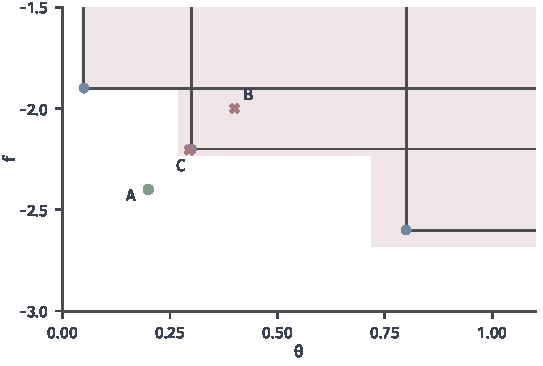
\includegraphics[width=92mm]{figures/05-optimization/06-constrained-optimization/matplotlib/sqp-filter-plane/figure.pdf}
 \caption{过滤器的$(\theta,f)$平面，蓝点是三条记录，深灰线是它们支配的范围边界，红色浅底是带裕量$\gamma=0.1$的禁止区。绿点$A$被接受，红叉$B$和$C$被拒绝，其中$C$虽不被支配，但在裕量带内。}
 \label{fig:sqp-filter-plane}
\end{BookInlineFigure}

\paragraph{还需要什么}
只靠式~\eqref{eq:sqp-filter}并不足以保证收敛到KKT点。还要回答三件事。

第一，局部切换。若迭代点已经几乎可行，而模型预测目标有明显下降，就不能只凭$\theta$有所改善就接受，要转而要求目标满足类似式~\eqref{eq:sqp-armijo}的充分下降，这样的步也不写入过滤器。否则算法可能收敛到一个可行但并不最优的点。

第二，什么时候写入记录。不满足上述切换条件而被接受的步，把当前点的$(\theta,f)$写入过滤器，并删去被它支配的旧记录。这样禁止区只会扩大，同一区域不会被反复光顾。

第三，可行性恢复。回溯到很小的步长仍无法被接受，说明当前的线性化方向帮不上忙，这时转入下一节的恢复阶段。过滤器不能代替这些规则。

表~\ref{tab:sqp-merit-filter}总结了两种规则。

\begin{BookInlineTable}
 \centering
 \begin{tabular}{lll}
  \toprule
  比较项 & 罚函数 & 过滤器\\
  \midrule
  进展的度量 & 一个数$\phi_\rho$ & 两个数$(\theta,f)$\\
  需要的参数 & 权重$\rho$ & 裕量$\gamma$、切换常数\\
  主要风险 & $\rho$太小或太大 & 需额外的恢复与切换\\
  历史信息 & 不保存 & 保存记录\\
  \bottomrule
 \end{tabular}
 \caption{罚函数线搜索与过滤器的比较。}
 \label{tab:sqp-merit-filter}
\end{BookInlineTable}
